
\chapter{Implementierung}
\section{OAuth2}
\subsection{Frontend}
\begin{figure}[H]
  \centering
  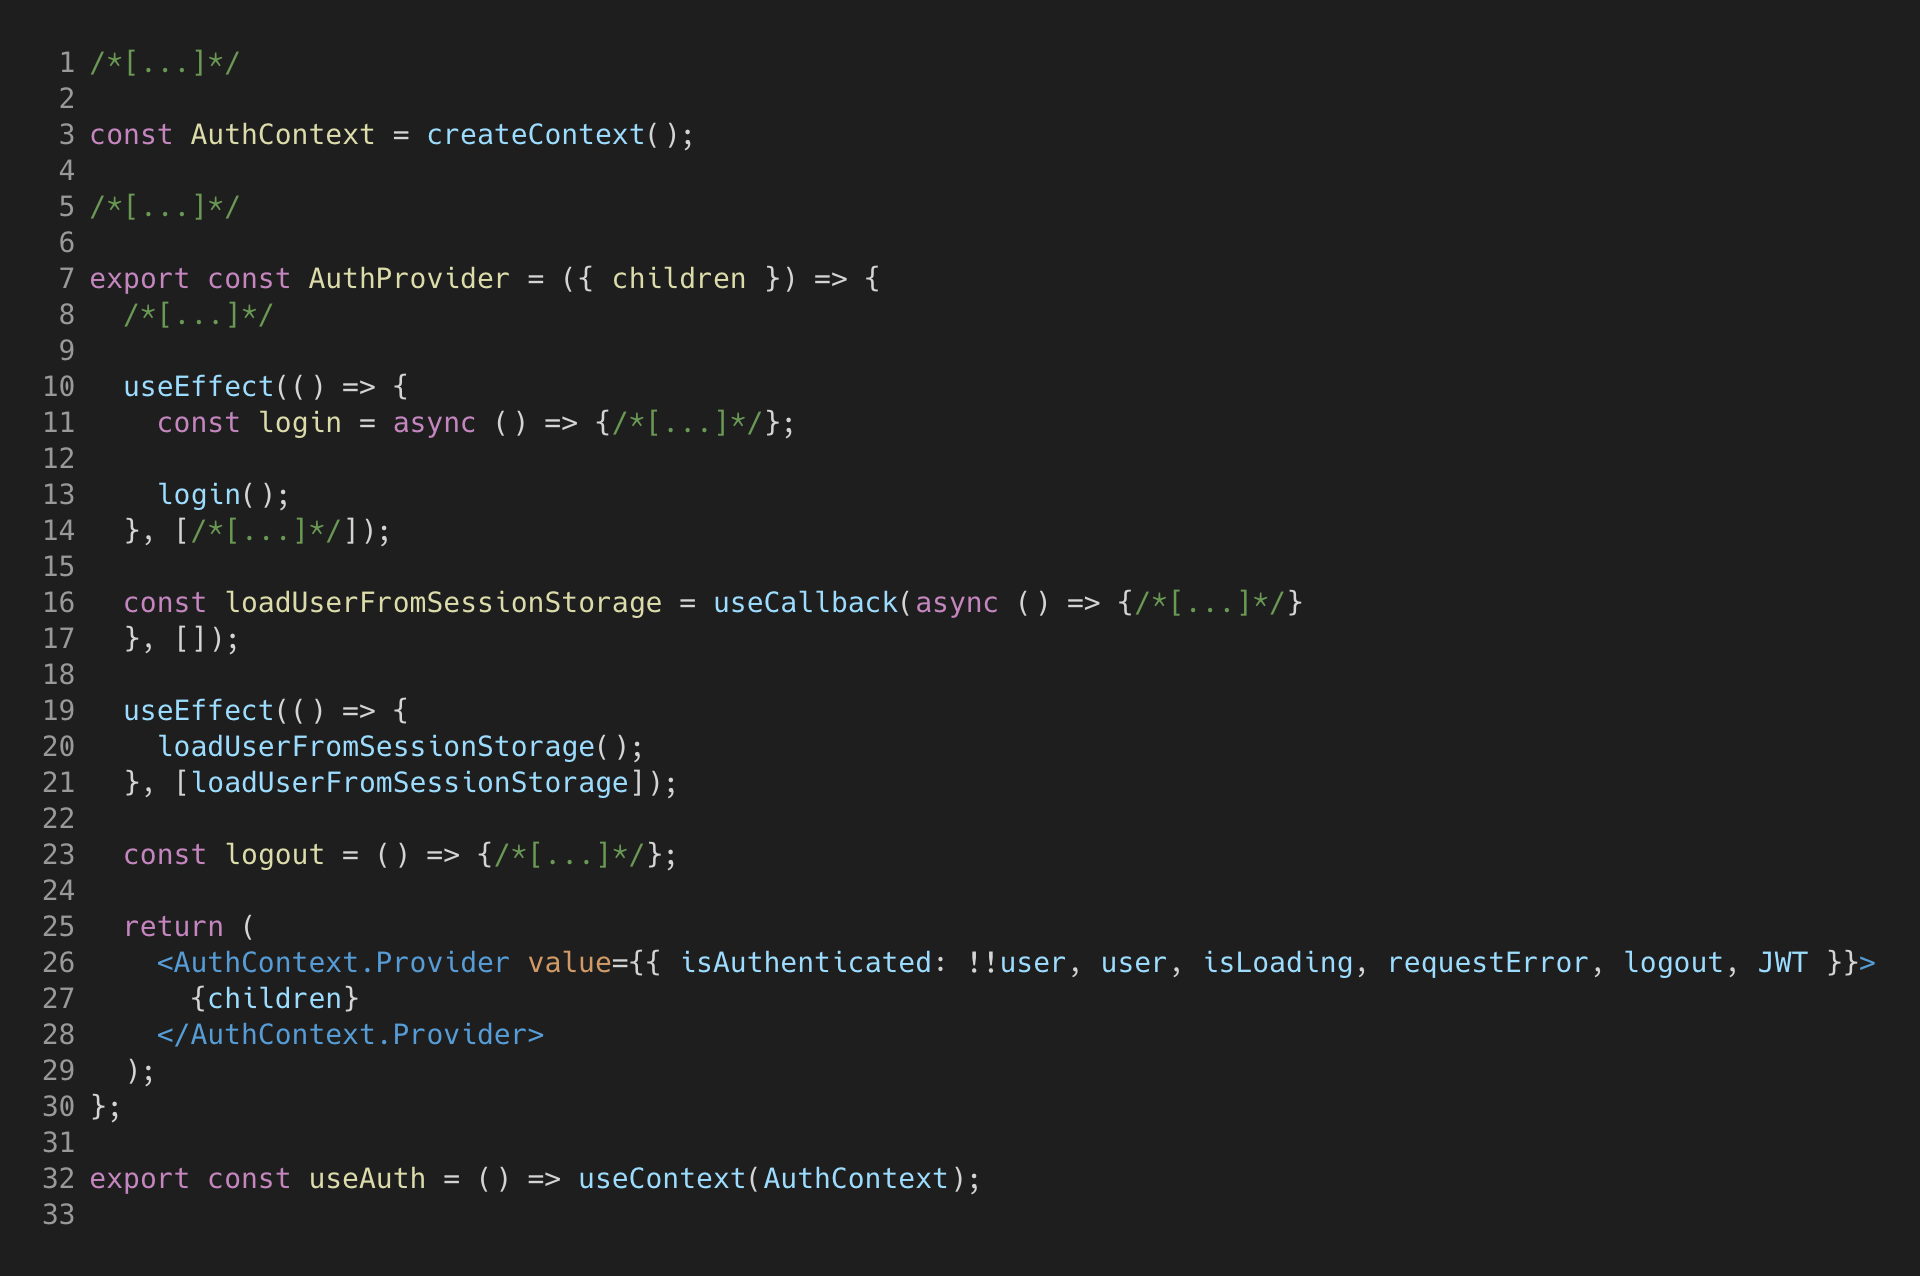
\includegraphics[width=.95\linewidth]{./images/authContext.png}
  \caption[{authContext.js von \code{ose-dashboard-frntnd}}]{authContext.js von \code{ose-dashboard-frntnd}}
  \label{fig:authContext}
\end{figure}
Dinge wie der JWT, Nutzerinformationen oder Funktionen wie \amk{login} und \amk{logout} müssen global in der Nextjs Applikation zur verfügung stehen. Vor ein paar Jahren hätte man dies noch mit Redux lösen müssen. Mittlerweile gibt es allerdings in React ein Konzept mit dem Namen \amk{Context}. Context erlaubt es einem, einen Wrapper mit State und Funktionen zu schreiben und diese den Subkomponenten zur verfügung zustellen. Werden Nutzerinformationen oder dazugehörige Funktionen in einer Subkomponente verwendet, können diese mit der \code{useAuth} Hook konsumiert werden. Dies sieht wie folgt aus:
\begin{figure}[H]
  \centering
  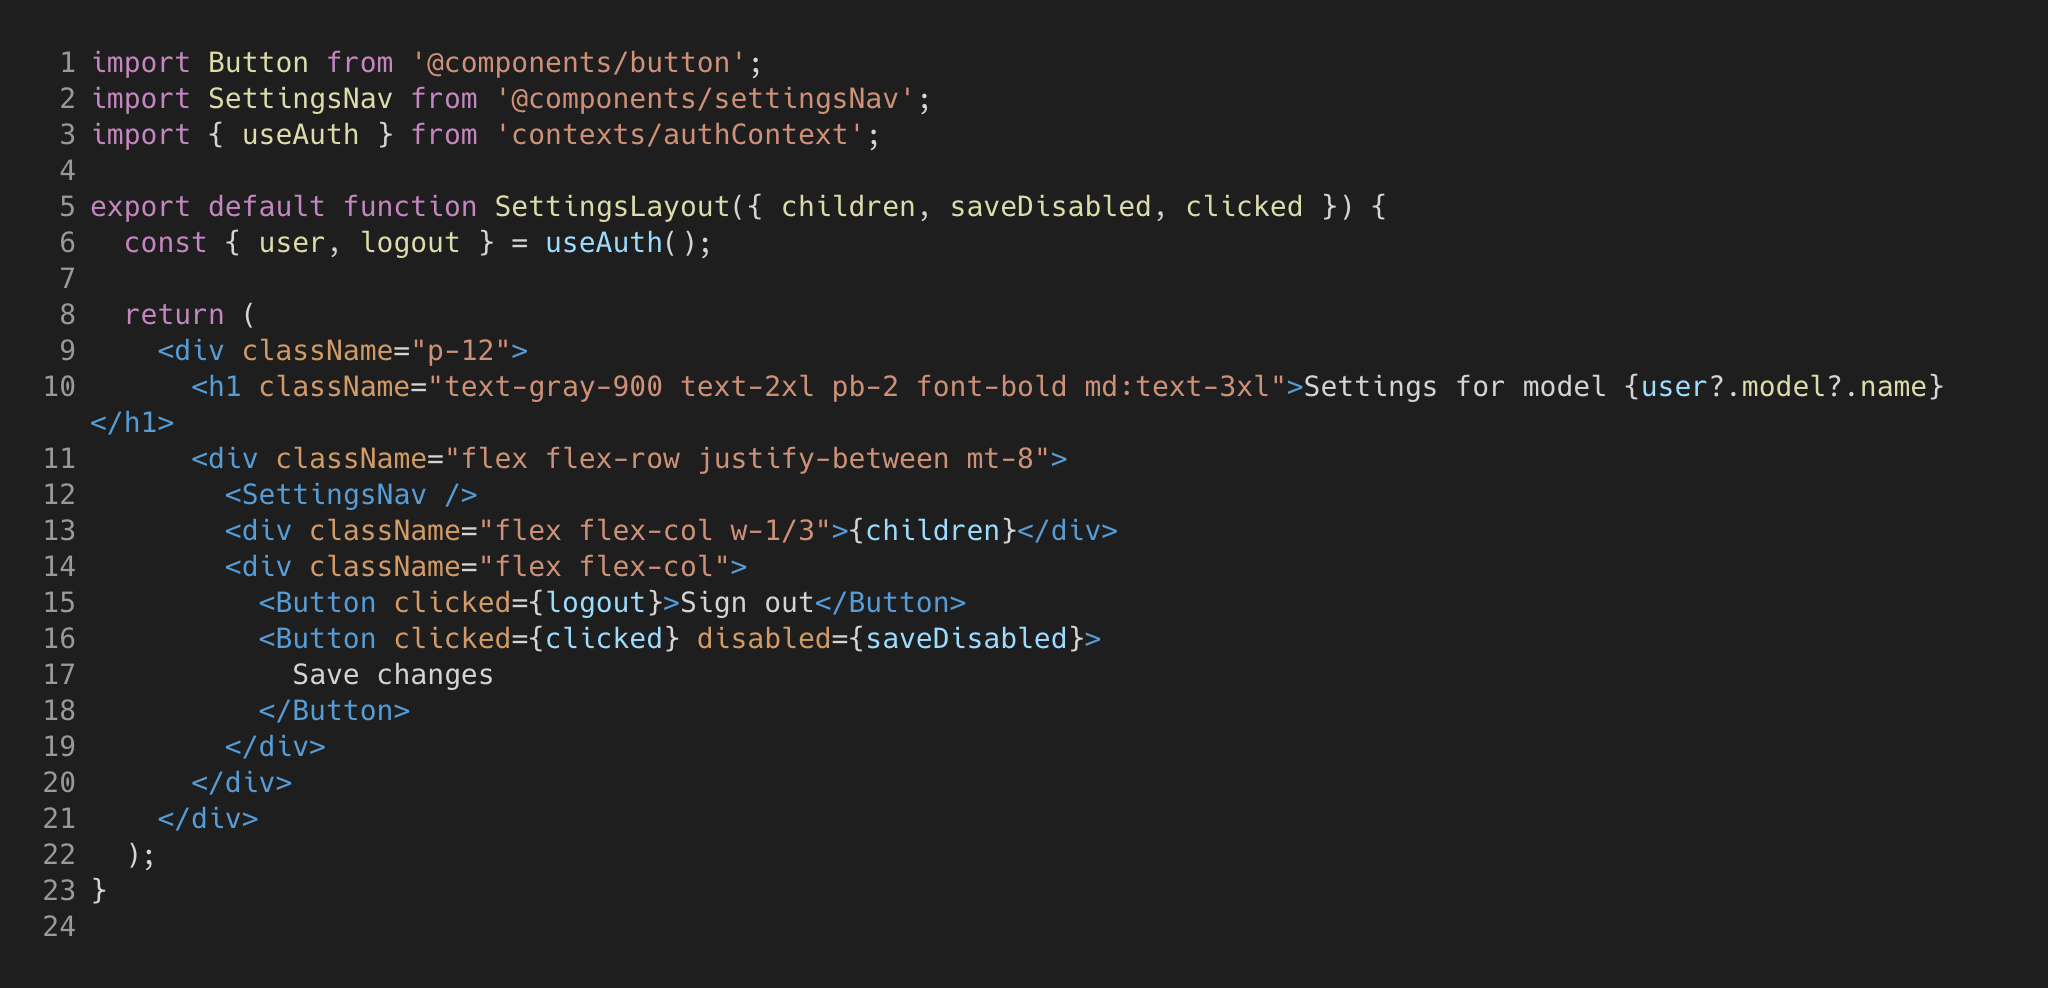
\includegraphics[width=.95\linewidth]{./images/settingsLayout.js.png}
  \caption[{settingsLayout.js von \code{ose-dashboard-frntnd}}]{settingsLayout.js von \code{ose-dashboard-frntnd}}
  \label{fig:settingsLayout}
\end{figure}
In der Zeile 6 wird der \amk{user} und die \amk{logout} Funktion vom Context konsumiert. Dies ermöglicht das anzeigen des Namen des Modelles auf Zeile 10 und das abmelden auf Zeile 15.
\subsection{Backend}
Der schwierige Teil der Implementierung von OAuth2 befindet sich allerdings im Backend. Eine Bedingung ist, dass sich der Nutzer anmelden kann. Die Zweite ist, dass alle Modelle in einem Intervall die Daten ihrer Assets aktualisieren. Diese Funktionalitäten sind in den beiden nachfolgenden Kapiteln beschrieben.
\subsubsection{Log-in}
\begin{figure}[H]
  \centering
  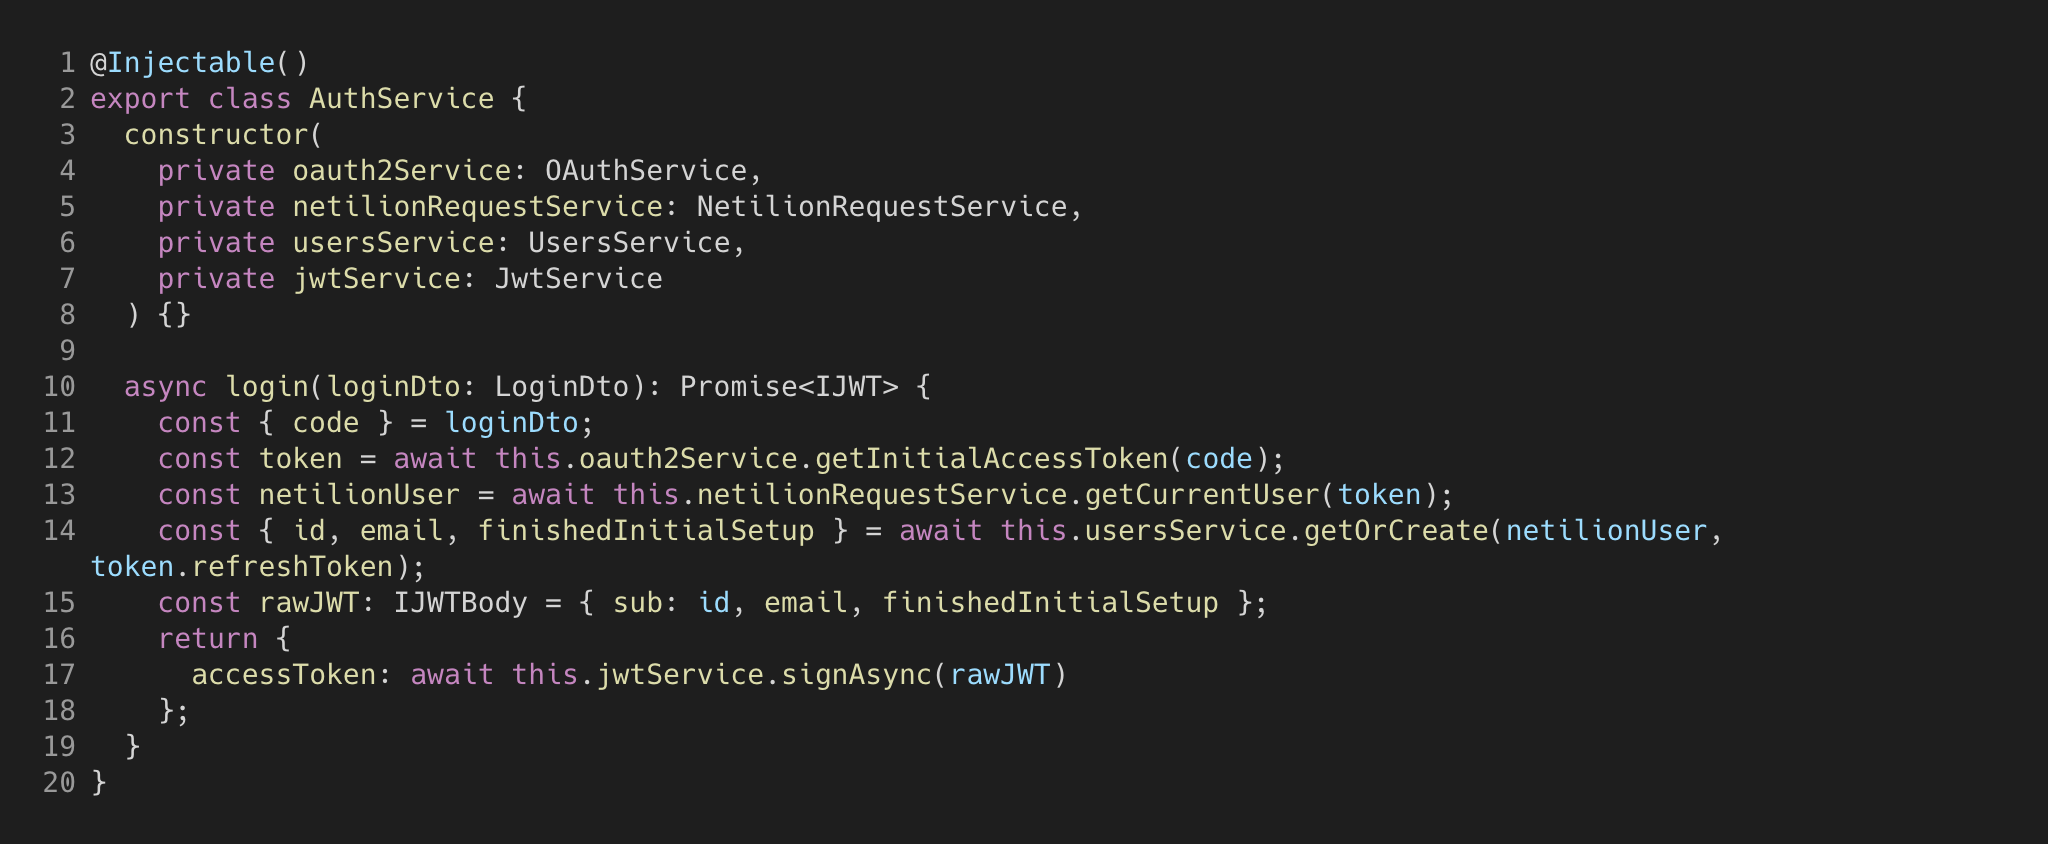
\includegraphics[width=.95\linewidth]{./images/auth.service.ts.png}
  \caption[{auth.service.ts von \code{ose-dashboard-bcknd}}]{auth.service.ts von \code{ose-dashboard-bcknd}}
  \label{fig:auth-service}
\end{figure}
Das Frontend erhält bei einer erfolgreichen Anmeldung einen Code. Dieser Code sendet es weiter an das Backend. Als erstes wird der Code in einen Token umgewandelt. Mit diesem Token ist es nun möglich die Nutzerinformationen von Netilion abzufragen. Anschliessend wird die Function \code{getOrCreate} vom \code{usersService} mit den Nutzerinformationen und dem Token aufgerufen. Diese Funktion fragt zuerst bei der Datenbank nach, ob der Nutzer bereits existiert. Existiert er, wird er direkt zurückgeben. Existiert er nicht, wird ein neuer erstellt.
Danach werden die für den JWT-Payload nötigen Daten in einem Objekt gebündelt und vom \code{jwtService} in einen signed JWT formattiert.
\newline
Der JWT wird als Antwort auf die Anfrage zurück ans Frontend gesendet, wo er fortlaufend, wie in Kapitel \ref{andwendung-jwt} beschrieben, als Authentifizierungsmethode zwischen Front- und Backend verwendet wird.
\subsubsection{Assets}
\begin{figure}[H]
  \centering
  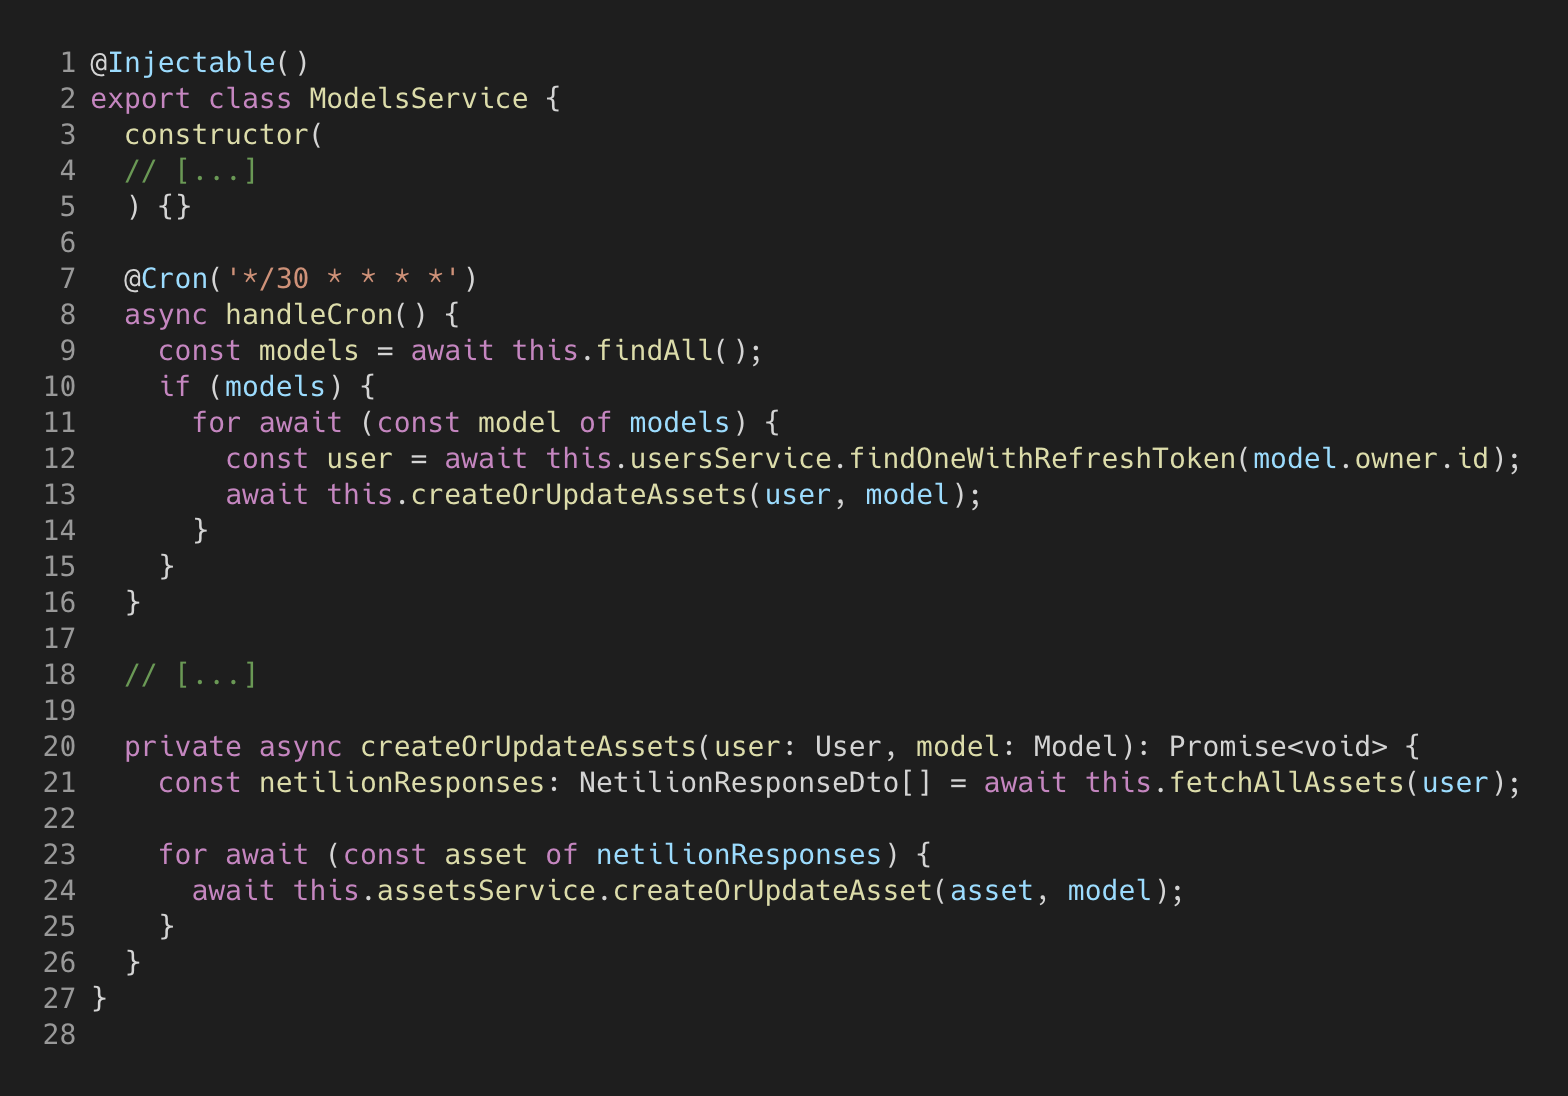
\includegraphics[width=.95\linewidth]{./images/models.service.ts.png}
  \caption[{models.service.ts von \code{ose-dashboard-bcknd}}]{models.service.ts von \code{ose-dashboard-bcknd}}
  \label{fig:models-service}
\end{figure}
Im \code{ModelsService} ist von Zeile sieben bis 16 ein Cron-Job deklariert. Dieser ist so konfiguriert, dass die \code{handleCron} Funktion auf Zeile acht alle 30 Minuten aufgerufen wird. Diese Funktion fragt zuerst beim Repository alle Modelle nach. Anschliessend wir in einer Schleife von jedem Modell der dazugehörige Nutzer abgefragt, womit danach die Funktion \code{createOrUpdateAssets} aufgerufen wird.
\newline
Diese Funktion fragt zuerst bei Netilion nach allen Assets des Users nach. Nachdem die Antwort erhalten wurde, schleift sie über alle Assets und ob diese erstellt werden müssen oder einfach aktualisiert werden können.
\section{Account löschen}
Normalerweise kann man sich bei einem Dienst wieder abmelden und dank GDDPR auch alle seine Daten löschen lassen. In unserem Fall sollte der \code{refresh\_token} des OSE-Verantwortlichen revoked werden, woraufhin die Entität gelöscht wird. Im optimalen Falle sollte das ORM so konfiguriert sein, dass danach alle Daten kaskadierend gelöscht werden. Das bedeutet, dass alle Einträge in der Datenbank, welche mit dem User in Verbindung gebracht werden können, nacheinander gelöscht werden.
\newline
Da dies ein bedeutender Auwand ist, welcher nicht von dieser IPA verlangt wird, werde ich dies nach der Abschlusspräsentation implementieren.
\section{Modellauswahl}
Es wurde schon bei Kapitel \ref{mck:index} auf die Abbildung \ref{fig:mck-index} eingegangen, dabei wurde jedoch ein Punkt bewusst weggelassen. Die Fläche, welche mit \amk{Model selection} markiert ist, soll nicht einfach leer sein, sondern dem Nutzer das Navigieren der Modelle einfach zu machen.
\newline
Bei den Mockups wurde allerdings das ganze noch nicht verfeinert, da mögliche Lösungen zuerst evaluiert werden sollen. Momentan stehen zwei Möglichkeiten zur Auswahl bereit. Diese werden in den Kapiteln \ref{mdlauswl-a} und \ref{mdlauswl-b} beschrieben.
\subsection{Auflistung mit Landesflaggen} \label{mdlauswl-a}
Die initiale Idee der Modellauswahl war eine Auflistung der Modelle nach den Ländern. Damit ich dies im Frontend machen kann, muss ich zuerst im Controller der Modelle eine neue Route implementrieren, welche sie nach den Ländern geordnet zurücksendet.
\newline
Meiner Meinung nach ist diese Möglichkeit sehr simpel, was nicht negativ gemeint ist. Sollte ich merken, dass die andere Möglichkeit Probleme macht oder machen könnte, werde ich diese implementieren.
\subsubsection{Pro}
\begin{itemize}
  \item Einfach zu implementieren
  \item Erfüllt den Zweck
  \item Lauft etwas schief, kann ich mir selbst weiterhelfen
\end{itemize}
\subsubsection{Kontra}
\begin{itemize}
  \item Eine dynamische Darstellung von Flaggen, in der Form von Bildern oder Emojis, könnte sich als schwieriger als Gedacht herausstellen
  \item Schwierig schön darzustellen
  \item Mehr Fleissarbeit um dies zu implementieren
\end{itemize}
\subsection{Interaktive Weltkarte} \label{mdlauswl-b}
Eine Idee die von mir kommt, ist die Darstellung mit einer Weltkarte. Ich hatte diese Idee bevor die IPA begann und habe mich in der Freizeit weiter informiert. Zuerst dachte ich, ich könne eine Karte im SVG-Format nehmen und selbst eine solche React-Komponente erstellen. Schnell wurde klar, dass sich dies als sehr grosser Aufwand herausstellen würde. Dadurch begann ich mit der recherche nach Libraries von Dritten, welche sich diese mühe bereits gemacht haben. Somit stiess ich auf \href{https://www.react-simple-maps.io/}{\code{react-simple-maps}}.
\newline
Mit dieser Komponente ist es mir möglich, eine Weltkarte mit Markern darzustellen. Die Marker werden dabei mit Koordinaten gesetzt. Da ich bei der Registration die Koordinaten des Modells erhalte, sollte dies kein Problem sein.
\subsubsection{Pro}
\begin{itemize}
  \item Ohne Konfigurationen sieht diese Komponente schön aus
  \item Weniger Fleissarbeit um dies zu implementieren
\end{itemize}
\subsubsection{Kontra}
\begin{itemize}
  \item Ich muss mich etwas in die Dokumentation einlesen
  \item Lauft etwas schief, kann mir nur Google oder die Dokumentation weiterhelfen
\end{itemize}
\subsection{Tatsächliche Auswahl}
Bei der Implementierung wird nun zweitere Möglichkeit, welche in Kapitel \ref{mdlauswl-b} beschrieben wurde, implementiert. Grund dafür ist, dass genügen Zeit zur verfügung ist und nicht eine overengineerte Lösung gebastelt werden muss, welche kurz nach der IPA ersetzt wird. Begründet wird dieser Entscheid damit, dass die Dokumentation im Aspekt der Verwendung in diesem Projekt gründlich durchgelesen wurde. 
\section{Automatische Verlinkung von Assets und Meshes}
Eine Anforderung dieser IPA ist, dass die Verlinkun von Assets und Meshes automatisch gemacht werden kann. Dies ist möglich, da sich bereits alle benötigten Informationen in der Datenbank des Backends befinden. Dies soll so die Erfahrung des Benutzer fördern und den Registrationsprozess vereinfachen.
\begin{figure}[H]
  \centering
  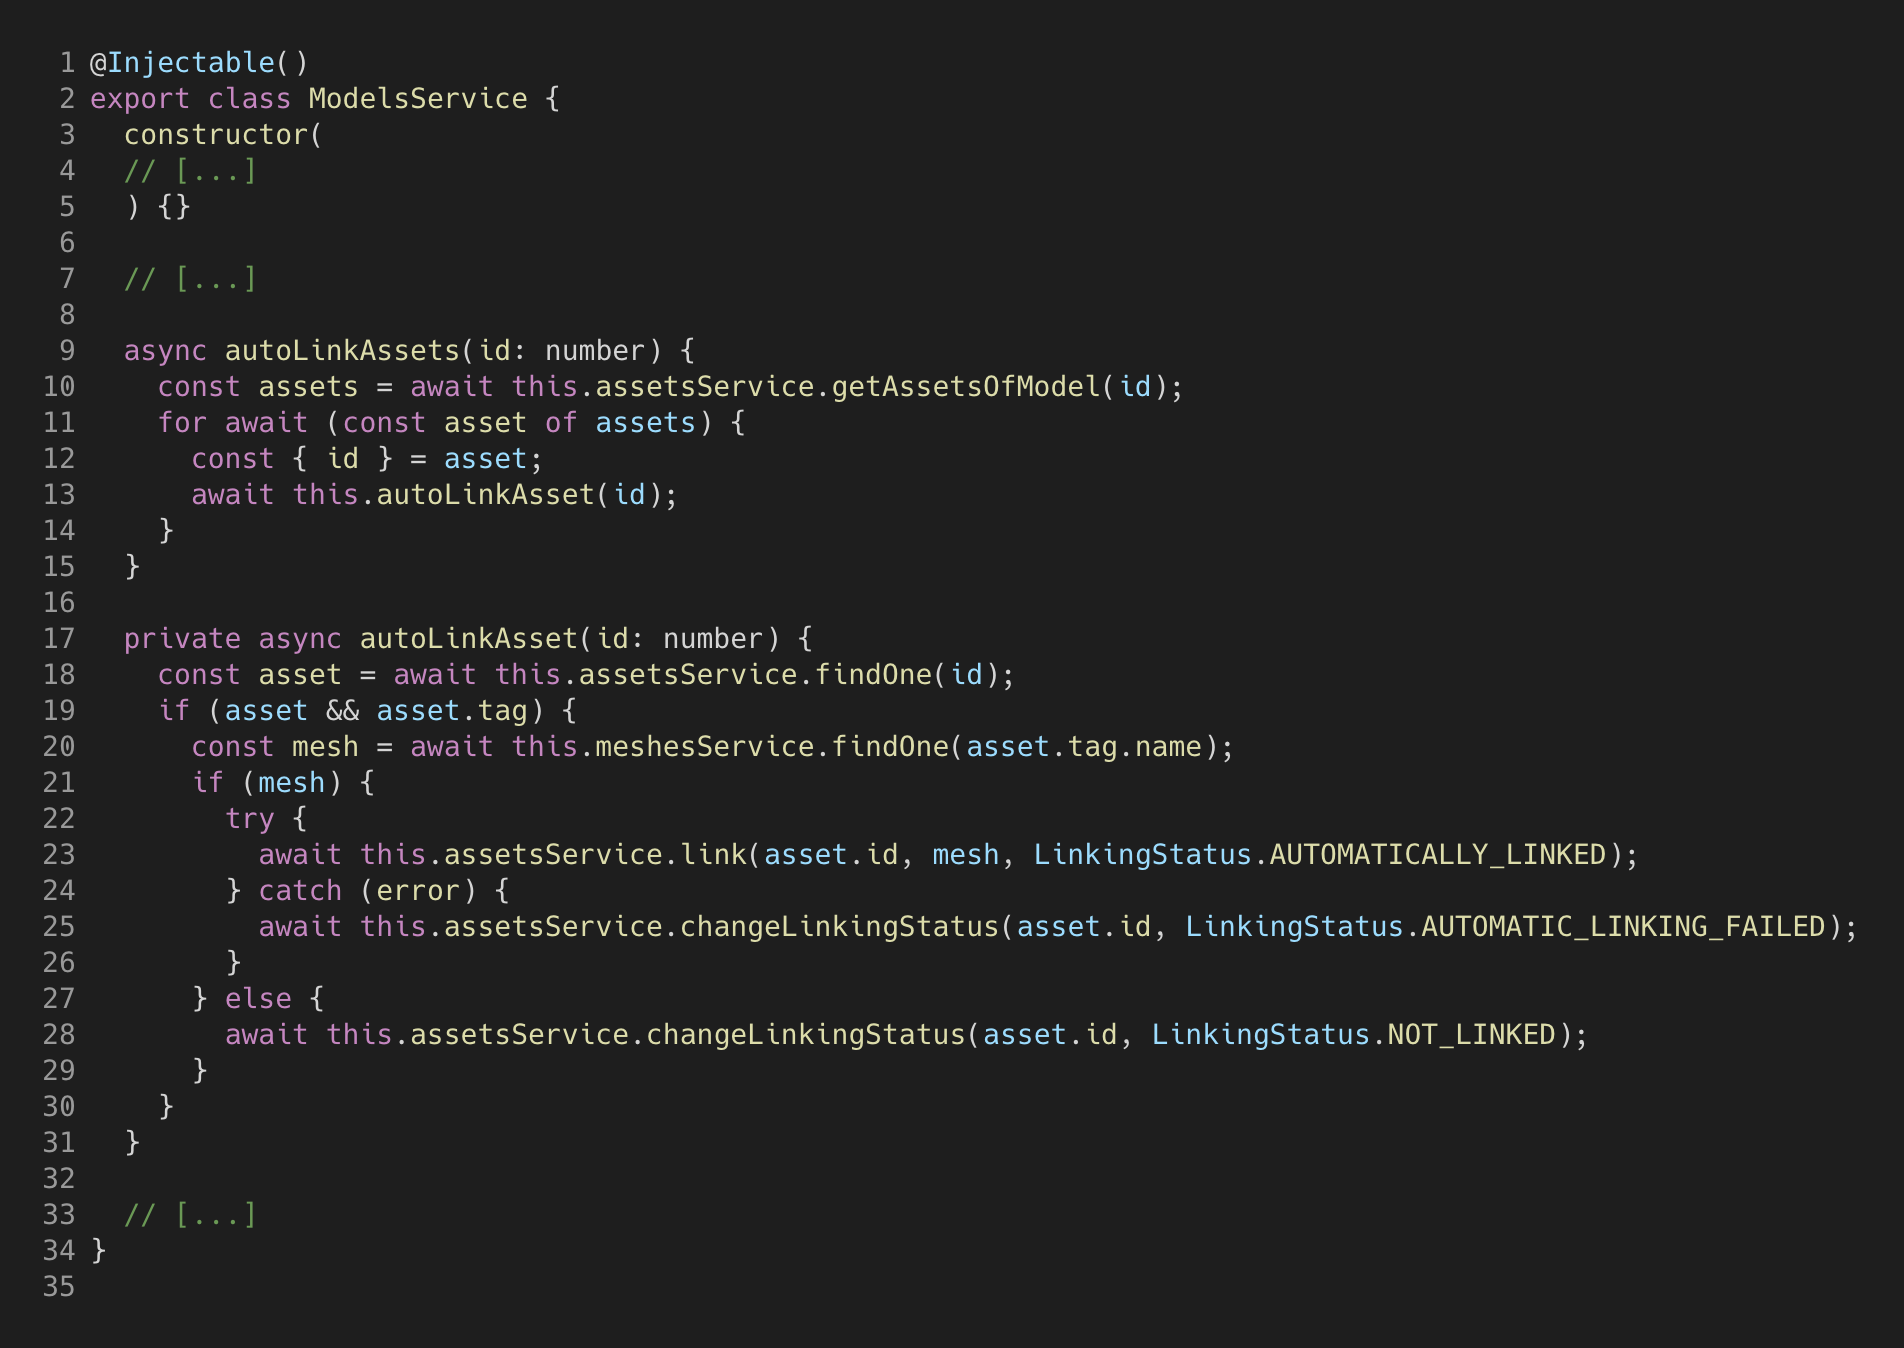
\includegraphics[width=.95\linewidth]{./images/models.service.ts.2.png}
  \caption[{models.service.ts von \code{ose-dashboard-bcknd}}]{models.service.ts von \code{ose-dashboard-bcknd}}
  \label{fig:settingsLayout}
\end{figure}
Die Funktion \code{autoLinkAssets} schleift über alle Assets eines Modells und ruft dabei für jedes einzelne \code{autoLinkAsset} auf. Diese erstellt die wirkliche Verlinkung. Dafür fragt es das Asset zuerst einzeln beim \code{assetsService} nach, da auf diesem Weg die Relation zu \code{Tag} left joined und selektiert wird. Wurde ein Asset mit einem Tag gefunden, wird beim \code{meshesService} nachgefragt, ob ein Mesh mit dem Namen des Tags existiert. Ist dies der Fall, werden die beiden miteinander verlinkt.
\section{Einhaltung der Coding Guidelines}
Die Coding Guidelines wurden eingehalten. Der Linter zeigt auf dem Front- und Backend weder Errors noch Warnings an. Es ist wichtig zu erwähnen, dass die Regeln nicht angepasst wurden und es keine Instanz gibt, an der eine Regel ignoriert wurde.
\newline
Dies kann bei beiden Repositories mit dem Kommand \code{yarn lint} überprüft werden.
\begin{figure}[H]
  \centering
  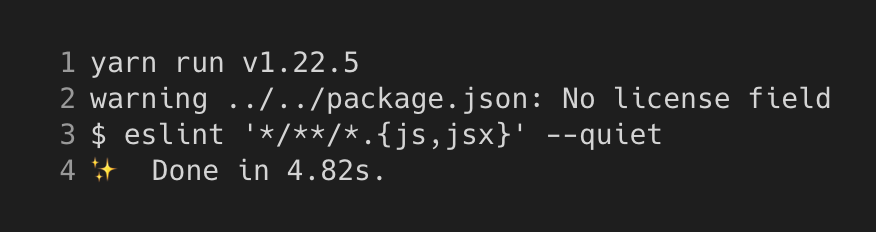
\includegraphics[width=.7\linewidth]{./images/linting-frontend.png}
  \caption[{Output von \code{yarn lint} im Frontend}]{Output von \code{yarn lint} im Frontend}
  \label{fig:lint-frnt}
\end{figure}
\begin{figure}[H]
  \centering
  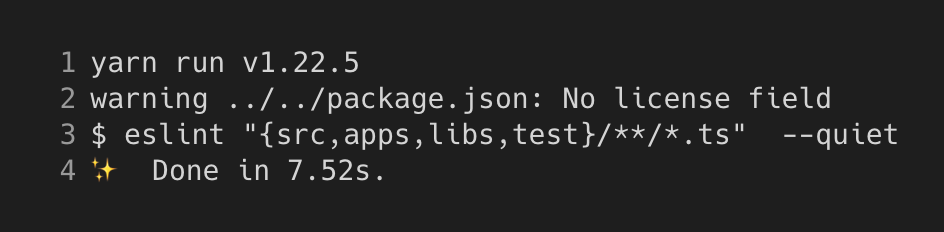
\includegraphics[width=.7\linewidth]{./images/linting-backend.png}
  \caption[{Output von \code{yarn lint} im Backend}]{Output von \code{yarn lint} im Backend}
  \label{fig:lint-bck}
\end{figure}
Eine Anmerkung muss hierbei gemacht werden. Die \amk{Warning} die in den Abbildungen \ref{fig:lint-frnt} und \ref{fig:lint-bck} bezieht sich nicht auf das Linting. Es handelt sich dabei um eine Warnung des Packetmanagers \amk{NPM}. Dieser wirft die Warnung, da ihm die Lizens in der Datei \code{package.json} unbekannt ist. Da es sich bei dieser Arbeit um kein öffentliches Projekt handelt, habe ich \code{\amk{license}: \amk{UNLICENSED}} angegeben.
\section{Umgebungsvariablen}
Umgebungsvariablen sind für fast alle Webanwendung nötig. Sie machen es möglich geheime oder heikle Daten der Anwendung erst zur Laufzeit zur Verfügung zu stellen. Auf diese Weise müssen die Daten nicht im Code fest angegeben werden. So kann ein Versionskontrollsystem eingesetzt werden, ohne das Dritte an heikle Daten kommen. Folgend sind die verwendeten Umgebungsvariablen beschrieben.
\subsection{Umgebungsvariablen - Frontend}
\begin{table}[H]
  \begin{tabularx}{\textwidth}{X X}
  \textbf{Variable} & \textbf{Beschreibung} \\ \\\hline \\
  NEXT\_PUBLIC\_AUTH\_URL & Die URL, auf die der Benutzer während dem Anmeldeprozess weitergeleited wird \\
  NEXT\_PUBLIC\_API\_BASE\_URL & URL, welche auf eine Instanz des Backends zeigt. \\
  \\\hline
  \end{tabularx}
\end{table}
\subsection{Umgebungsvariablen - Backend}
\begin{table}[H]
  \begin{tabularx}{\textwidth}{X X}
  \textbf{Variable} & \textbf{Beschreibung} \\ \\\hline \\
  PORT & Der Port unter dem das Backend erreichbar ist \\
  DATABASE\_URL & Datenbankverbindungsadresse \\
  NETILION\_AUTHURL & Basis URL für Anfragen an den OAuth2 Endpoint \\
  NETILION\_AUTHURL & Basis URL für Anfragen an den OAuth2 Endpoint \\
  NETILION\_URL & Basis URL für Anfragen an die Resourcen Endpoints \\
  NETILION\_REDIRECT\_URI & URI, auf die der User nach dem Anmeldeprozess weitergeleited wird \\
  NETILION\_CLIENT\_ID & Id der erstellten OAuth2 Applikation in Netilion \\
  NETILION\_CLIENT\_SECRET & Secret der erstellten OAuth2 Applikation in Netilion \\
  REDIS\_URL & Redis Verbindungsadresse \\
  REDIS\_TTL & Gibt an, wie lange Einträge in Redis gespeichert bleiben \\
  SECURITY\_JWT\_SECRET & String, mit welchem die JWTs signiert werden \\
  SECURITY\_JWT\_EXPIRES\_IN & Gibt an, wie lange JWTs gültig sind \\
  SECURITY\_JWT\_EXPIRES\_IN & String, mit welchem die \code{refresh\_token} verschlüsselt werden \\
  GEOLOCATION\_API\_KEY & Zugriffsschlüssel, um auf die \amk{HERE Developer API} zugreifen zu können \\
  PERMITTED\_USERGROUP\_ID & Id der Netilion UserGroup. Nur die darin enthaltenen Nutzer können sich anmelden \\
  PERMITTED\_USERGROUP\_NAME & Name der Netilion UserGroup. Nur die darin enthaltenen Nutzer können sich anmelden \\
  \\\hline
  \end{tabularx}
\end{table}
\section{3D Modell auswechseln}
In der ersten Version des OSE-Dashboards stellte sich die korrekte Einbindung des Modells als schwierig heraus. Grund dafür ist, dass die Datei mehrmals mit speziellen konfigurationen umgewandelt werden muss. Diese Schritte sind in diesem Kapitel beschrieben, damit nachfolgende Entwickler/-innen sich die Mühe und Zweit ersparren können.
\begin{enumerate}
  \item Das Model wird von einem Konstrukteur von Endress+Hauser erstellt. Da Konstrukteure CAD-Modelle modellieren, wird die Datei mit hoher wahrscheinlichkeit vom Typ .stp sein.
  \item Wird ein Auftrag beim Konstrukteur erstellt, muss dieser darauf hingewiesen werden, dass die einzelnen Bestandteile des Modells für uns korrekt benannt werden müssen. Im Schritt 10 ist es sehr wichtig, dass die Benennung keine Umlaute (öäü) und Leerzeichen enthält.
  \item Für die erste Umwandung wird das Program \amk{FreeCAD} verwendet. Dieses muss auf einem Windows Computer installiert werden.
  \item Die .stp Datei importieren und als .dae exportieren
  \item Für die nächste Umwandung brauchen wir eine 3D Modellierungssoftware. Bisher wurde Blender verwendet, da dies keine Kosten verursacht.
  \item In Blender kann das Modell nun nach belieben angepasst werden. Zum Beispiel können Farben verändert werden.
  \item Anschliessend soll das Modell als .gltf exportiert werden. In diesem Schritt kann der Detailgrad bestimmt werden. Je höher der Detailgrad desto grösser ist die Datei. Eine grosse Datei verlangsamt die Ladezeit erheblich und erfordert moderne Hardware um flüssig angezeigt werden zu können.
  \item Nun kann die .gltf Datei in den \amk{public} Ordern von React/Nextjs gelegt werden. Dies ist notwendig, da der Client des Benutzers diese Datei herunterladen können muss.
  \item Für den nächsten Schritt brauchen wir ein Script. Das Repository dafür ist \href{https://github.com/pmndrs/gltfjsx}{\code{pmndrs/gltfjsx}}. Dieses muss nicht installiert werden, sondern kann als Remote Script mit NPM ausgeführt werden. In der Dokumentation des Scriptes ist die korrekte Anwendung beschrieben.
  \item Nun sollte mit gltfjsx aus der .gltf Datei eine React Komponente generiert werden. Diese sollte in den \amk{components} Ordner verschoben werden.
  \item Um das Modell darzustellen, muss das Modell in der Scene Komponente eingebunden werden.
  \item Damit das Modell interaktiv wird, müssen noch einige kleine konfigurationen gemacht werden. Die Szene enthält eine Variable \amk{assetSelected}. Diese muss der Modell Komponente als property weitergegeben werden.
  \item Anschliessend müssen die Meshes im Modell, welche ein Asset darstellen, durch die Komponente \amk{Asset} ersetzt werden und mit zusätzlichen Informationen ausgestattet werden. Dies wird in der Abbildung \ref{fig:mdl-cmpnt} dargestellt.
\end{enumerate}
\begin{figure}[H]
  \centering
  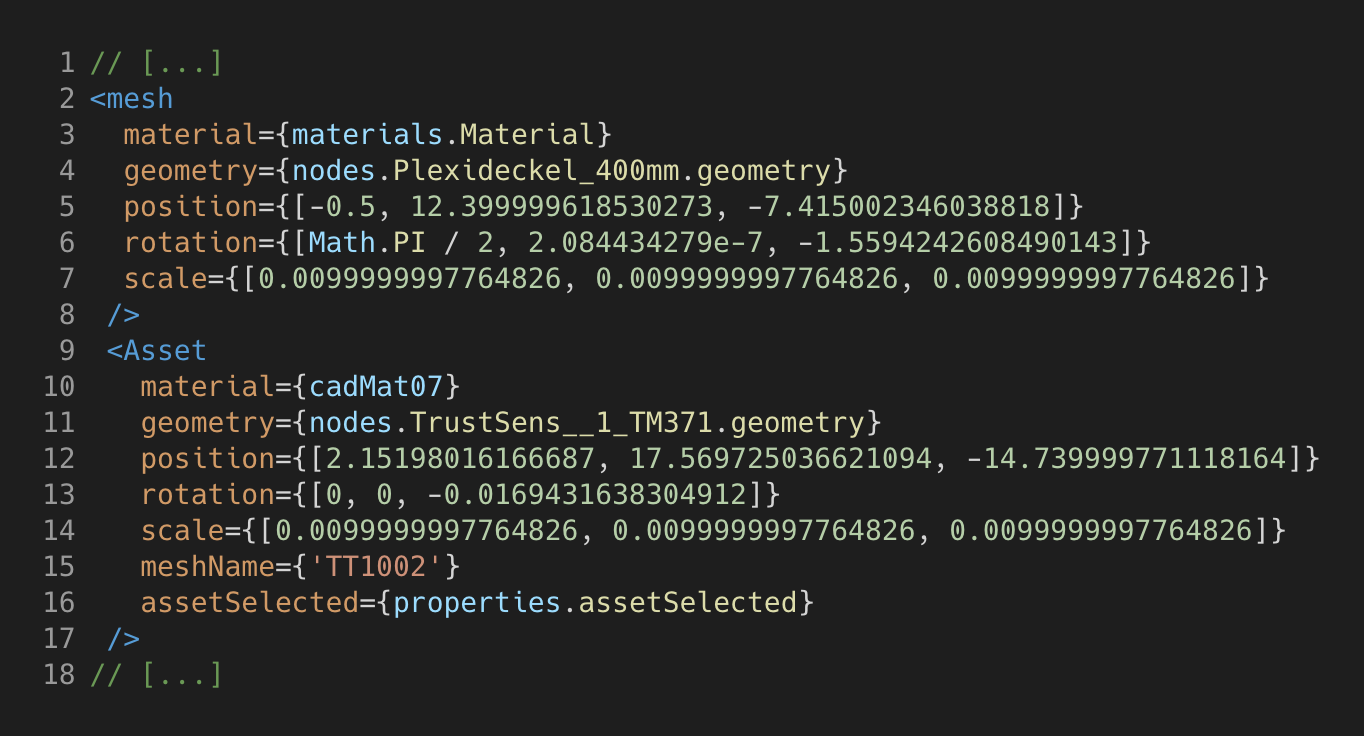
\includegraphics[width=.7\linewidth]{./images/model.js.png}
  \caption[{Ausschnitt aus der momentanen \amk{Model.js} Komponente}]{Ausschnitt aus der momentanen \amk{Model.js} Komponente}
  \label{fig:mdl-cmpnt}
\end{figure}
Die \amk{Asset} Komponente besteht aus einem Mesh. Daher werden auch alle Properties des Meshes verlangt. Zusätzlich muss der Mesh mit einem Tag benannt werden. Damit die hierarchisch höher liegende Komponente erkennen kann, wann welches Asset angeklickt wurde, muss noch die Funktion \amk{assetSelected} mitgegeben werden.

Mit diesem Schritt ist die einbundung eines neuen Modelles abgeschlossen.
